\listfiles
\documentclass[a4paper, abstracton]{scrartcl}
\usepackage[utf8]{inputenc}
\usepackage{amsmath, amsfonts, enumerate}
\usepackage{graphicx}		% graphics
\usepackage[colorinlistoftodos]{todonotes}
\usepackage{hyperref}		% enables the usage of links
\usepackage{glossaries}		% glossary
\setlength{\parindent}{0pt} 	% disable padding of first sentence in a paragraph
\setlength{\parskip}{11pt}		% disable gap between parapgraphs
\usepackage{fixltx2e}		% enables textsubscripting
\usepackage{fancyhdr}		% used for page layout
\usepackage{caption}
\usepackage{subcaption}
\usepackage{float}
\usepackage{listings}		% http://ctan.org/pkg/listings

\lstset{
  basicstyle=\ttfamily,
  mathescape
}

% add font of scrartcl / koma: -> european writing style, wider pages and so on. See def. of KOMA / scratcl
\addtokomafont{author}{\normalsize} 
\addtokomafont{date}{\normalsize} 
%\setkomafont{disposition}{\bfseries}

\setlength{\headheight}{48pt}

% style of all other pages
\fancypagestyle{basicpagestyle}{
	\fancyhf{}								% clear everything
	\fancyfoot[C]{\thepage}
	\renewcommand{\footrulewidth} {1pt}		% set rule thickness
	\renewcommand{\headrulewidth} {1pt}
	\rhead{Bern University of Applied Sciences}
	\lhead{
\includegraphics[width=0.8cm]{images/BFHlogo.png}}
	% \fancyfoot[L]{}
	% \fancyfoot[R]{}

}

% style of first page
\fancypagestyle{titlepage}{
   \fancyhf{}
   \renewcommand{\footrulewidth} {0pt}		% set rule thickness
   \renewcommand{\headrulewidth} {1pt}
   \lhead{
\includegraphics[width=0.8cm]{images/BFHlogo.png}} %  add logo
   \fancyhead[R]{Bern University of Applied Sciences} % text
}

\pagestyle{basicpagestyle}

\begin{document}
\title{\vspace{1cm}AWT Bookmaker \vspace{1cm}}
\author{
  Stefan Andonie\\
  \texttt{andos1@students.bfh.ch}
  \and
  Pascal Grüter\\
  \texttt{grutp1@students.bfh.ch}\vspace{1cm}
}

\date{Biel, \today}
\vspace{3cm}
\maketitle
\thispagestyle{titlepage}

%\includegraphics[width=15cm]{images/titlepage.jpeg}

\pagebreak
\tableofcontents	% add table of contents (takes 2x typesetting to generate)
\pagebreak

\section{Einleitung}

  Für das Semesterprojekt im Modul Advanced Web Technologie wurde ein Wettsystem
  als Webapplikation implementiert.
  Das System wurde mit Java Server Faces realisiert und soll auf einem Apache
  Tomcat Applikationsserver laufen.
  
  Das Wettsystem soll es einem Buchmacher erlauben Fussballspiele zu erfassen
  und Wettzenarien für gewisse Ergebnisse und Ereignisse währen eines Spiels mit
  dazugehörigen Wettquoten zu definieren.
  Danach sollen Spieler Wetten darauf abschliessen können.

\section{Architektur}

  Unsere Implementierung folgt dem Model, View, Controller Pattern.
  Die Views wurden wie üblich mit JSF in den xhtml Files definiert.
  Diese Views werden jeweils von einem Java Bean gesteuert, das ist der
  Controller Teil. Die Buissneslogik befindet sich getrennt in eigenen Java
  Klassen die unser Domainmodel abbilden und auf welche die Controller zugreifen.
  
  Die Daten bzw. die Instanzen der Domainklassen werden mit Hilfe eines ORMappers
  (Hibernate, JPA) an eine Relationelle Datenbank angebunden und so persistiert.

  \subsection{Projektstruktur}

  Dieses Pattern findet sich in der Struktur des Projektes wider.
  Im Sourceverzeichnis finden wir die "bookmaker" und die "model" Package und
  ausserhalb das Webverzeichnis, es enthält die Views und deren Ressourcen
  und die JSF Konfiguration.
  Die Bookmakerpackage enthält sämtliche Controllers und einige Hilfsklassen und
  Methoden die es erlauben Properties und Objekte zu laden oder Objekte zu
  manipulieren und zu speichern.
  Dort werden die Ausgabewerte für die Views berechnet und das System bedient.
  Die Modelpackage enthält die Domainmodel Klassen. Die darin enthaltene
  Buissneslogik erlaubt es Benutzer und Wetten zu erstellen und Wetten
  abzuschliessen. Hier wird der Zustand des Systems abgebildet.
  Des Weiteren befinden sich im Sourceverzeichnis die mehrsprachigen Propertiesdateien und weitere Konfigurationsdateien wie die Konfiguration vom Hibernatecontroller.
  
\pagebreak

\section{Model}
 
  Unser Domainmodel
  (Siehe Abbildung \ref{fig:domain_model} auf Seite \pageref{fig:domain_model})
  beinnhaltet folgende Klassen.
  
  \subsection{User}
    Der User enthält sämtliche Eigenchaften eines Benutzers wie
    den vollständigen Namen, Emailadresse, Logininformationen und den eine Variable für das Spielgeld. Der User hat eine Rolle, er ist entweder
    Bookmaker oder Gambler. Da es nur diese zwei Rollen gibt wurde dem User
    ein Boolean Attribut gegeben welches ihn als Bookmaker ausweist fall es
    true ist. Der Bookmaker sieht die von ihm erstellten Spiele.
    Als Bookmaker können neue Spiele erfasst werden und alte Spiele müssen
    geschlossen werden. Als Bookmaker kann aber nicht gewettet werden.
    Der Gambler kann nun auf diese Spiele wetten aber selber keine Spiele
    erfassen. Der Gambler sieht eine Liste der Spiele auf welcher er gewettet hat.
      
  \subsection{Game}
    Ein Spiel beinhaltet die id der Teams und eine Liste von Conditions.
    Jedes Spiel hat ein Datum und eine Zeit wann es beginnt.
    Die Teamnamen sind als mehrsprachiger String in den Propertiesdateien mit einer
    id gespeichert.
    Wenn ein Spiel begonnen hat darf nicht mehr darauf gewettet werden.
    Das Spiel enthält einen boolean der true ist falls das spiel abgeschlossen
    wurde (closed). Ein Spiel ist abgeschlossen falls mindestens 90min nach
    der Anfangszeit der Bookmaker der es erstellt hat die Conditions
    auswählt welche eingetroffen sind (occurred).
      
  \subsection{Condition}
    Conditions sind Ereignisse die während eines Games eintreffen können.
    Sie gehören immer zu einem Game.
    Sie beinhalten eine Textid eines mehrsprachigen Textes und Parameter
    die in den Text eingefügt werden, sowie eine Wettquote (odd).  
    Die Conditions enthalten des weiteren einen boolean der anzeigt ob
    sie eingetroffen (occurred) ist (true) oder nicht (false).
    Dieses Attribut soll beim Beenden eines Spieles vom Bookmaker gesetzt
    werden. Anschliessend kann bestimmt werden wer gewonnen hat.
     
  \subsection{Bet}
    Bets können vom Gambler erstellt werden.
    Bets enthalten eine Condition auf die gewettet wird und einen Betrag
    der vom Gambler eingesetzt wird. Der Betrag wird beim erstellen vorläufig
    dem Gambler abgezogen. Wenn ein Spiel beendet wurde erhält der Gambler
    einen Gewinn der dem Einsatz multipliziert mit der Wettquote entspricht
    vom Bookmaker falls die Condition eingetroffen ist. Oder sonst erhält der Bookmaker den Einsatz. 

  \begin{figure}[h!]
  \begin{center}
    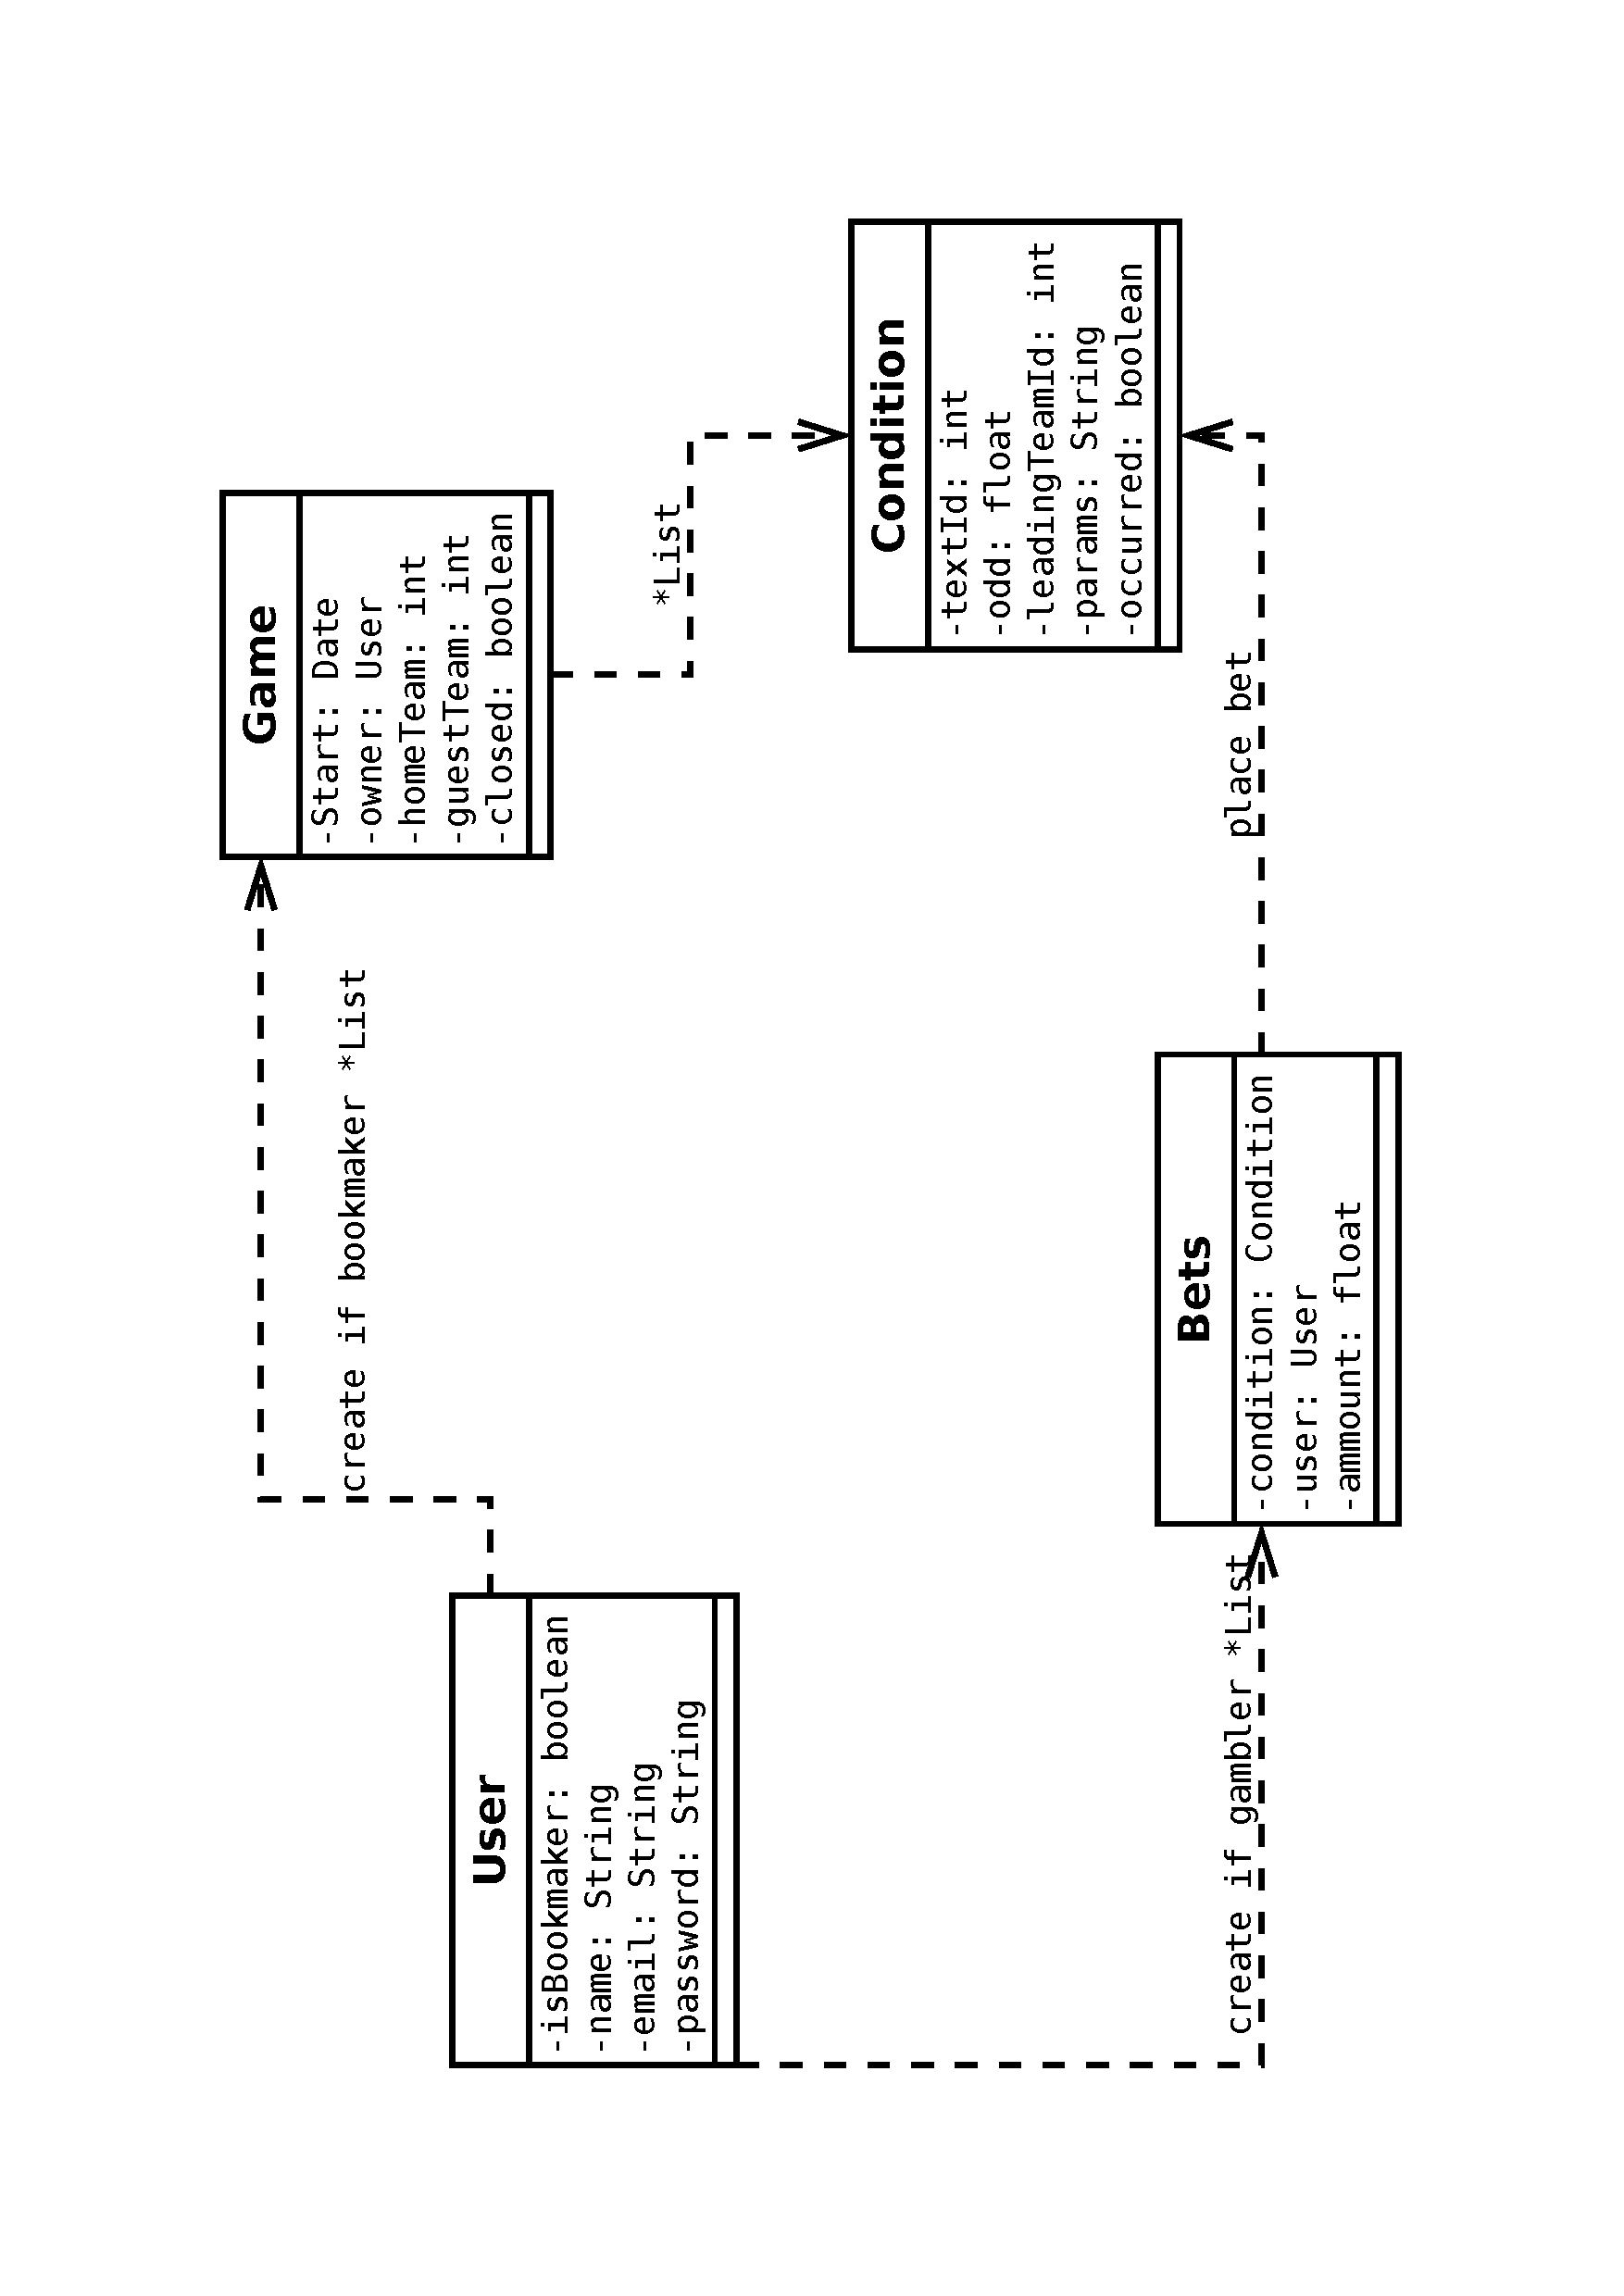
\includegraphics[width=0.7\textwidth,angle=-90]{images/DomainModel.pdf}
  \end{center}
  \caption{Domain Model}
  \label{fig:domain_model}
\end{figure}

\subsection{Hibernate}
  Um die Objekte in einer Datenbank zu persistieren haben wir Hibernate und eine
  MySql Datenbank benutzt. Hibernate ist ein Object Relation Mapper (ORM) und
  ermöglicht es Javaobjekte auf relativ einfache weise in ein relationeles
  Model zu übersetzen. Pro Objekt wird eine Tabelle erstellt, diese Relation Beinhaltet
  die Attribute des Objekts die primitive Datentypen sind oder Strings.
  Attribute Die widerum selber Objekte sind weden über foreign keys gemappt.
  Listen werden mit einer vielfach beziehung dargestellt.
  Für die Datenbank wurde noch eine Objektid als primary key zu den Objekten
  hinzugefügt.
  Das daraus resultierende Datenbankmodel ist in
  Abbildung \ref{fig:db_model} auf Seite \pageref{fig:db_model} zu sehen.


\begin{figure}[h!]
  \begin{center}
    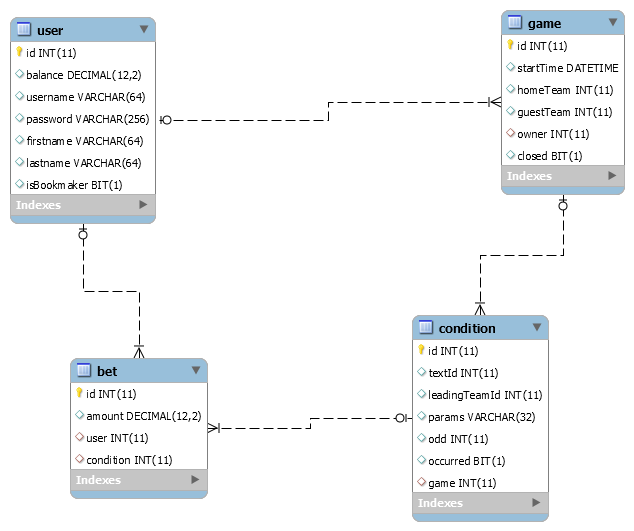
\includegraphics[width=0.7\textwidth]{images/db_model.png}
  \end{center}
  \caption{Datenbank Model}
  \label{fig:db_model}
\end{figure}

\section{Views und Controller}

  Die Views sind so aufgebaut dass sie jeweils aus einer äusseren und einer
  inneren View zusammen gesetz sind. Das wurde mit ui:insert und ui:composition
  realisiert.
  
  Die äussere View, das basetemplate, bleibt für jede Seite gleich, sie beherbergt
  die Navigation und das login/logout. Die Navigation wird abhängig davon ob ein User eingeloggt
  ist und dessen Rolle im Sessionbean zusammen gestellt.
  
  Die inneren Views entsprechen dem Content der auf der jeweiligen Seite
  angezeigt werden soll.
  
  Jede View entspricht einem Usecase und wird durch ein Bean gesteuert.


\subsection{Sessionbean}
  Das Sessionbean implementiert das login und speichert den aktuellen Benutzter.
  Bevor sich ein Benutzter einloggt wird ein lehrer User erstellt damit ein Gast
  einige Innhalte wie zum Beispiel eine liste mit Spielen sehen kann oder auf die
  registrationform kommt.
  Ausserdem wird hier die Sprache geladen.
  
  Das SessionBean enthält auch eine Methode zu erzeugung von Hibernate Sessions
  damit Objekte gespeichert und aktuallisiert werden können.
  
  Des weiteren kann vom Sessionbean auch eine Instanz der Hilfsklasse PropertiesUtil
  geladen werden. Diese Hilfsklasse erlaubt es die in Properties files gespeicherten
  Texte der Conditions und Teamnamen in der jeweiligen Sprache als java Map 
  oder einen Einzelnen Text per id zu laden.
  Das wird beim erstellen eines Spieles benötigt wo der Benutzer aus einem Dropdown
  Teams und Conditions auswählen soll.
  
\subsubsection{Navigation}
  Die Navigation besteht aus Links zu den jeweiligen Seiten, einem Menu um die
  Sprache zu ändern und einem Formular um sich einzuloggen bzw. auszuloggen.
  
  Die Navigation wird im Sessionbean zusammen gestellt. Dafür gibt es eine innere
  Klasse NavLink weleche das Label und das Ziel eînes Links beinhaltet.
  Diese NavLinks werden in einer Liste verwaltet. Für einen Besucher der nicht
  eingelogt ist stehen nur einige Links zu verfügung. Beim einloggen und ausloggen
  werden jenach Rolle des Nutzters Links hinzugefügt oder entfernt.
  Danach wierden die Links neu geladen in der Methode reloadNavlinks, hier müssen
  die labels aus den bundels geladen werden.
  Die Links werden im baseTemplate mit hilfe eines ui:repeats aus der Liste auf
  der Seite dargestellt.

\subsection{balance}
  Ein zweistuffiges Formular um auf den Spielkredit des Users eizuzahlen.
  Die erste Form Dient dazu eine Kreditkarte zu Validieren.
  Dazu wird eine 16 stellige kartennummer in vier viererblöken eingegeben
  und ein dreistelliger validierungscode.
  Dabei handelt es sich um ein Mockup, es wird lediglich die nummer
  1234-1234-1234-1234 und der code 234 akzeptiert.
  Danach erscheint eine Eingabe auf der der einzuzahlende Betrag angegeben wird. 

\subsection{closeGame}
  Hier werden die vom Bookmaker erstellten Spiele bei welchen die Startzeit
  90 min zurückliegen angezeit. Der Bookmaker sollt nun diese Spiele beenden.
  Er wählt dazu ein Spiel aus und gelangt in eine detailierte Ansicht.
  Über checkboxes kann er nun diejenigen Conditions ankreuzen die während dem
  Spiel aufgetreten sind. Danach schliesser das Spiel indem er auf den dafür
  vorgesehenen Button klickt.
  Bei den Objekten Game und Condition werden nun die Attribute closed bzw occurred
  gesetzt und in der Datenbank aktualisiert.

\subsection{games}
  Auf dieser Seite werden Die Spiele des Users angezeigt.
  Beim Gambler die Spiele auf die er gewettet hat einmal eine Liste laufender Spiele
  und eine Liste mit abgeschlossenen Spielen.
  Beim Bookmaker werden die von ihm erstellten Spiele angezeigt.
  Aus einer Tabelle können einzelne Spiele ausgewählt werden und in einer Detail
  Ansicht dargestellt werden. Es werden Die Teams angezeigt die Spielzeit und
  eine Tabelle mit Conditions.
  
  Für den Bookmaker sind hier die Beträge ersichtlich die er gewint bzw verliert,
  falls eine Condition eintritt oder nicht.
  
  Der Gambler sieht für noch laufende Spiele für jede Condition einen Input und
  einen Button. Er kann hier eine Summe eintippen und bestätigen das er auf diese
  Condition wettet. Der Gambler muss über den zu wettenden Einsatz verfügen.
  Für Spiele die beendet wurden wird Angezeigt ob die Condition eingetroffen ist
  und der Betrag der darauf von Gambler gewettet wurde.

\subsection{home}
  In der Home View werden alle laufenden Spiele aufgelistet.
  Bei jedem Spiel kann in eine Deail ansicht gewechselt werden.

\subsection{newGame}
  Hier kan der Bookmaker ein neues Spiel erstellen.
  Diese Ansicht besteht aus zwei formularen. wir haben die rendered option der form
  benutzt um eine Game erfassung in zwei Stuffen zu realisieren.
  zuerst müssen die Teams und die Zeit angegeben werden. Die Teams werden aus den
  properties viles geladen und können anschliessend in einem Dropdown für das Home-
  und Guestteam selektiert werden. Die Zeit kann per Datepicker angegeben werden 

  Danach wird auf die Ansicht zum erstellen von Conditions gewechselt.
  Die Conditions werden Stückweise zusammengefügt aus Mehrsprachigen Texten und
  Parametern. Der Vorteil liegt darin das die Mehrsprachigkeit gegeben Bleibt.
  Ausserdem kann kontrolliert werden welche Wetten erlaubt sind und einigermassen
  Sinn machen.
  Über ein Dropdown kann nun das eines der vorher ausgewählten Teams selektiert
  werden. Über das nächste dropdown kann nun der mehrspracige text ausgewählt werden.
  Eine Hilfsmethode erlaubt es die Anzahl parameter im Text festzustellen,
  Entsprechend viele Inputfelder werden generiert. Die Parameter werden als
  Kommaseparierter String gespeichert. Beim Darstellen der Condition werden diese
  separiert und können die placeholder ersetzen generiert.
  Ebenfalls muss eine Wettquote angegeben werden.
  Die Condition wird über ein Ajax event erstellt wenn der entsprechende Button
  gedrückt wurde. In einer Tabelle werden die erstellten Conditions dargestellt
  und können noch gelöscht werden.
  Der bookmaker kan nun das Speil erstellen, es kann danach nicht mehr geändert werden.
  
\subsection{registration}
  Ein Simples registrierungsformular um einen User zu erfassen. Es werden alle nötigen
  Angaben erfasst, Vor- und Nachname, Emailadresse sowie ein Passwort das noch
  einmal bestätigt wird.
  Danach werden Serverseitig die Eingaben geprüft insbesondere die länge der Eingaben
  und ob die Passworter übereinstimmen und ein paar Regex.
  Das Passwort wird gehasht bevor es gespeichert wird.
  Der User wird als Gambler erstellt, er kann sich mit der Email adresse einloggen.
  Der Bookmaker wurde per Hand in der Datenbank erstellt bzw das isBookmaker
  flag auf true gesetzt.

\section{Fazit}


\pagebreak
\listoffigures		% add list of figures (takes 2x typesetting to generate)

\pagebreak	% see difference between pagebreak, newpage and clearpage


\pagebreak


\pagebreak	


\end{document}
